\documentclass{article}
\usepackage{cTex}
\usepackage{amssymb}
\usepackage{amsmath}
\usepackage{geometry}
\usepackage{threeparttable}
\usepackage{graphicx}
\geometry{left = 3.0cm, right = 3.0cm, top = 2.0cm, bottom = 2.0cm}
\title{这是我的第一份\LaTeX{}论文文档}
\author{Ruini Yang (yangruinii@foxmail.com) \\Department of Communication \\
UESTC,\ Chengdu,\ Sichuan, 611731}
\begin{document}
    {
        \maketitle
        \begin{center}
        \textbf{Abstract} \\
        \end{center}
        \qquad A user identity anonymity is an important property for roaming services. In 2011, Kang et al. proposed an improved user authentication scheme that guarantees user anonymity in wireless communications. This letter shows that Kang et al.'s improved scheme still cannot provide user anonymity as they claimed.\\
        \indent \emph{\textbf{Keywords:} \ cryptanalysis, authentication, anonymity, wireless communications, security} \\
\section{Introduction}
\noindent In 2004, Zhu and Ma \cite{Li10} proposed an authentication scheme with anonymity for wireless 
communication environments. Later, Lee et al. \cite{Zhang10} showed several security flaws of Zhu-Ma’s scheme and then 
improved it. However, in 2008, Wu et al. \cite{Lohr10} showed that both Zhu-Ma’s scheme and Lee et al.’s scheme still 
cannot provide anonymity and then proposed an improvement to preserve anonymity. Nevertheless, Zeng et al. 
\cite{WangWRL10} and Lee et al. \cite{Barsoum11} showed that Wu et al.’s scheme also cannot provide anonymity, respectively.\\ \indent In 2011, Kang et al. \cite{ZYan122} proposed an improved user authentication scheme based on both Wu et al.’s and 
Wei et al.’s schemes \cite{Lohr10}, \cite{Ateniese11} that guarantees strong user anonymity in wireless communications. However, this 
letter shows that the Kang et al.’s improved scheme also cannot provide user anonymity as they claimed.
    }
\section{Review of Kang et al.s Scheme}
\noindent Throughout the paper, notations are employed in Table 1. There are three phases in the Kang et al.'s scheme-initial phase, first phase, and second phase.\\
\begin{table}[h]
    \renewcommand{\tablename}{Table}
    \caption{Notation}
	% \label{Table 1}
    \centering
\begin{tabular}{|l|l|}
 \hline
 \emph{HA} & Home Agent of a mobile user \\ \emph{FA} & Foreign Agent of the network \\
 \emph{MU} & Mobile User \\
 \emph{${PW}_{MU}$} & A password of \emph{MU} \\
 \emph{N} & A strong secret key of \\
 \emph{${ID}_A$} & Identity of an entity \emph{A} \\
 $T_A$ & Timestamp generated by an entity \emph{A} \\
 \emph{${Cert}_A$} & Certificate of an entity \emph{A} \\
 \emph{$(X)_K$} & Encryption of message X using symmetric key \emph{K} \\
 \emph{$E_{P_A}(X)$ }& Encryption of message \emph{X} using public key of \emph{A }\\
 \emph{$S_{S_A}(X)$} & Signature on message \emph{X} using private key of \emph{A} \\
 \emph{$h(\cdot)$ }& A one-way hash function \\
 $||$ & Concatenation \\
 $\oplus$ & Bitwise exclusive-or operation \\
 \hline
  \end{tabular}
\end{table}
\subsection{Initial Phase}
Where an \emph{MU} registers with his/her \emph{HA}, the \emph{MU}'s identity $\emph{ID}_{\emph{MU}}$ is submitted to the \emph{HA}. After receiving $\emph{ID}_{\emph{MU}}$ from \emph{MU}, \emph{HA} generates $\emph{PW}_{\emph{MU}}$, $r_1$ and $r_2$ as follows. \\
%\begin{eqnarray}  
\begin{align}
    & PW_{MU} = h(N||ID_{MU}) \\
    & r_1 = h(N||ID_{HA}) \\
    & r_2 = h(N||ID_{MU}) \oplus {ID}_{MU}     
\end{align}
%\end{eqnarray}
where N is a secret value kept by \emph{HA}.\emph{HA} stores $\emph{ID}_{\emph{HA}}$, $r_1$, $r_2$ and $\emph{h}(\cdot)$ in the smart card of \emph{MU} and then sends it with $\emph{PW}_{\emph{MU}}$ to \emph{MU} through a secure channel.
\subsection{First Phase}
Figure 1 illustrates the first phase of Kang et al.’s scheme. A foreign agent \emph{FA} authenticates \emph{MU} 
by interacting with \emph{HA} as follows.
\begin{enumerate}
\item \emph{MU}$\rightarrow$ \emph{FA}:\{n,$(h({ID}_{MU})||{x_0}||x)_L$,${ID}_{HA},T_{MU}$\}\\
 If \emph{MU} inputs \emph{${ID}_{MU}$} and \emph{${PW}_{MU}$} to \emph{MU}'s mobile 
device chooses secret random values $x_0$ and x and computes \emph{n} and \emph{L} as follows.
    \begin{equation}
        n = h(T_{MU}||r_{1}) \oplus r_{2} \oplus PW_{MU}
    \end{equation}
    \begin{equation}
        L = h(T_{MU} \oplus PW_{MU})
    \end{equation}
     
    \emph{MU}'s mobile device sends \emph{MU}'s login message 
${n,(h({ID}_{MU})||x_0||x)_L,{ID}_{HA},T_{MU}}$ to \emph{FA},where \emph{$T_{MU}$} is a current 
timestamp.
\begin{figure}[htbp]
    \centering
    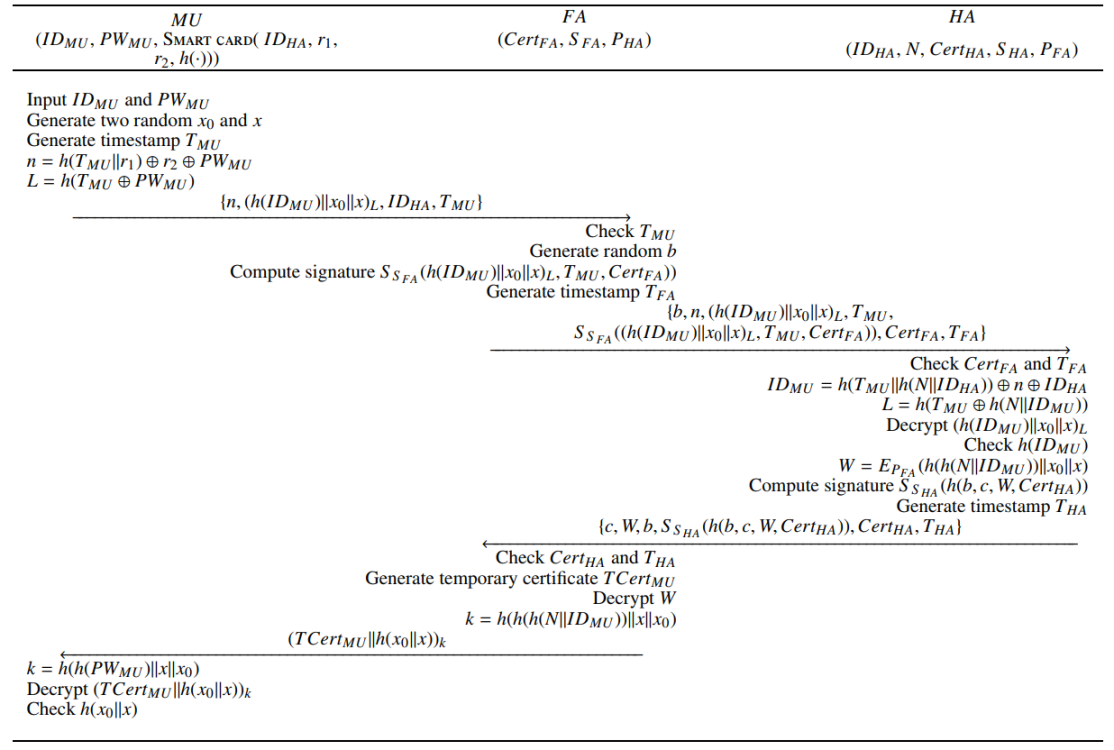
\includegraphics[width=5in]{figure.png}%重要
    \caption{First phase of Kang et al.'s scheme.}
    \end{figure}
\item \emph{FA}$\rightarrow$ \emph{HA}: 
$\{b,n,(h({ID}_{MU})||x_0||x)_L,T_{MU},{S}_{S_{FA}},((h({ID}_{MU})||x_0||x)_L,T_{MU},{Cert}_{FA}
),{Cert}_{FA},T_{FA}\}$\\
 FA checks the validity of $T_{MU}$. If it is valid, then FA chooses secret random number b. FA
 then sends b, the MU’s login message containing ${n,(h({ID}_{MU})||x_0||x)_L,{ID}_{HA}, T_{MU}}$, 
a certificate $Cert_{FA}$, timestamp $T_{FA}$, and the corresponding signature on the
 login message by using FA’s private key $S_{FA}$to HA.
%3
\item \emph{HA}$\rightarrow$ \emph{FA}: $\{c,W,b,S_{S_{HA} 
(h(b,c,W,{Cert}_{HA})),{Cert}_{HA},T_{HA}}\}$\\
 \emph{ HA} checks the validity of certificate $Cert_{FA}$ and timestamp $T_{FA}$. If they are valid, then 
\emph{HA }computes \emph{MU}’s real identity ${ID}_{MU}$ as follows.
\begin{equation}
    ID_{MU} = h(T_{MU}||h(N|| ID_{HA}))\oplus n \oplus ID_{HA}
\end{equation} 
 \emph{HA} computes \emph{$L = h(T_{MU}\oplus h(N||{ID}_{MU}))$} with his/hersecret \emph{N} 
and decrypts $(h({ID}_{MU})||x_0||x)_L$. Then, \emph{HA } verifies if \emph{MU} is a legal user by 
checking \emph{$h({ID}_{MU}) =h({ID}_{MU})'$} , where $h({ID}_{MU})$ is computed with 
\emph{${ID}_{MU}$} on the login message and $h({ID}_{MU})'$ of the decrypting result 
$\{h({ID}_{MU})'||{x_0}'||x'\}$. If so, then \emph{HA} computes $W 
=E_{P_{FA}}(h(h(N||{ID}_{MU}))||x_0||x)$ and generates its signature using his/her private key $S_{HA}$. 
Then, \emph{HA} sends random number $c, W$, the certificate of \emph{HA}, ${Cert}_{HA}$, current 
timestamp $T_{HA}$, and signature $S_{S_{HA}} (h(b,c,W,{Cert}_{HA}))$ to \emph{FA}.
\item \emph{FA}$\rightarrow$ \emph{MU}: $(T{Cert}_{MU}||h(x_0||x))_k$\\
 \emph{FA} checks whether or not the certificate ${Cert}_{HA}$ and timestamp $T_{HA}$ are valid. If 
they are valid, then \emph{FA} issues the emporary certificate $T{Cert}_{MU}$, which includes a timestamp 
and other information to \emph{MU}. To obtain $h(h(N||ID_{MU})||x_0||x)$, \emph{FA} decrypts \emph{W} 
with the secret key corresponding to $P_{FA}$. To establish session key $k_i$ for the \emph{i}-th session, 
\emph{FA} first saves $(T{Cert}_{MU}, h({PW}_{MU}),x_0)$. \emph{FA} encrypts 
$(T{Cert}_{MU}||h(x_0||x))$ with session key k and gives $(T{Cert}_{MU}||h(x_0||x))_k$ to \emph{MU}. 
Here, the session key is computed as follows.  
   \begin{equation}
    \begin{aligned}
        k & = h(h(h(N||ID_{MU}))||x||x_{0}) \\
          & = h(h(PW_{MU}))||x||x_{0}
    \end{aligned}         
    \end{equation}
    \item \emph{MU} computes \emph{k} and obtains $T{Cert}_{MU}$. \emph{MU} also authenticates 
\emph{FA} by computing $h(x_0||x)$ with the decrypted $h(x_0||x)$. Therefore, \emph{MU} can be sure that it 
is communicating with a legal \emph{FA}.
\end{enumerate}
\subsection{Second Phrase}
\noindent When \emph{MU} visits \emph{FA} at the \emph{i}-th session, \emph{MU} sends the following 
login message to \emph{FA}.
\begin{enumerate}
    \item \emph{MU} $\rightarrow$ \emph{FA}:$\text { TCert }_{M U},\left(x_{i}\left\|T C e r t_{M U}\right\| \text { OtherInformation }\right)_{k_{i}}$\\
    The new \emph{i}-th session key \emph{$k_i$} can be derived from the unexpired previous secret 
value\emph{$x_{i-1}$} and the fixed secret value \emph{x} as%
    \begin{equation}
        k=h\left(h\left(h\left(N \| I D_{M U}\right)\right)\|x\| x_{i-1}\right)
    \end{equation}
    where $i = 1,\ldots,n$.
    \item Upon receiving a login message from \emph{MU}, \emph{FA} decrypts $\left(x_{i}\left\|T C e r t_{M U}\right\| \text { OtherInformation }\right)_{k_{i}}$with $k_{i}$ and newly saves ($TCert_{MU}$,\emph{h($PW_{MU}$),$x_i$}) for the next communication.
\end{enumerate}

\section {Anonymity Problem of Kang et al.s Scheme}
\noindent Kang et al. \cite{ZYan122} improved Wu et al.’s scheme \cite{Lohr10} and Wei et al.’s scheme \cite{Ateniese11} to provide anonymity. 
Based on the general interest of mobile users, user anonymity should be kept from any eavesdroppers including 
the foreign agents \cite{Barsoum11}. However, Kang et al.’s scheme still cannot provide anonymity. The main reason is that 
\emph{HA} always computes r1for each \emph{MU} with the same secret key \emph{N}. The detailed 
anonymity broken attack scenario is as follows.

\begin{enumerate}
    \item Any legal user \emph{MU} can directly obtain $h(N||{ID}_{HA})$ from $r_1$ in his/her smart card 
    because $r_1=h(N||{ID}_{HA})$ from the Eq.(2)
    \item The legal user \emph{MU} can collect the messages $\left\{n^{\prime},\left(h\left(I D_{M U}^{\prime}\right)\left\|x_{0}^{\prime}\right\| x^{\prime}\right)_{L^{\prime}}, I D_{H A}, T_{M U}^{\prime}\right\}$ sent from any other legal mobile user 
    \emph{MU'} to \emph{FA} at step (1) in the first phase(see Fig.1).From the Eqs.(1)$\sim$(4),we can see that 
    \emph{n'} is equal to $h({T'}_{MU} ||r_1)\oplus {ID}_{HA}\oplus {ID'}_{MU}$ as follows.


\begin{equation}
    \begin{aligned}
        n^{\prime}=& h\left(T_{M U}^{\prime} \| r_{1}\right) \oplus r_{2}^{\prime} \oplus P W_{M U}^{\prime} \\
        =& h\left(T_{M U}^{\prime} \| r_{1}\right) \oplus h\left(N \| I D_{M U}^{\prime}\right) \oplus I D_{H A} \\
        & \oplus I D_{M U}^{\prime} \oplus P W_{M U}^{\prime} \\
        =& h\left(T_{M U}^{\prime} \| r_{1}\right) \oplus h\left(N \| I D_{M U}^{\prime}\right) \oplus I D_{H A} \\
        & \oplus I D_{M U}^{\prime} \oplus h\left(N \| I D_{M U}^{\prime}\right) \\
        =& h\left(T_{M U}^{\prime} \| r_{1}\right) \oplus I D_{H A} \oplus I D_{M U}
        \end{aligned}
\end{equation}
    \item With obtained $r_1=h(N||{ID}_{HA})$ and collected messages$\left\{n^{\prime}, I D_{H \Lambda}, T_{M U}^{\prime}\right\}$,\emph{MU} can get the real identity ${ID}^{\prime}_{MU}$ of the other mobile user $MU^{\prime}$ as \emph{HA} does at step(3) in 
the first phase as follows. 
\begin{equation}
    \begin{aligned}
        I D_{M U}^{\prime}=& n^{\prime} \oplus h\left(T_{M U}^{\prime} \| r_{1}\right) \\
        =& h\left(T_{M U}^{\prime} \| r_{1}\right) \oplus I D_{H A} \oplus I D_{M U}^{\prime} \\
        & \oplus I D_{H A} \oplus h\left(T_{M U}^{\prime} \| r_{1}\right) \\
        =& I D_{M U}^{\prime}
        \end{aligned}
\end{equation}
As a result, legal mobile user $MU^{\prime}\text{'s}$ anonymity cannot be preserved in Kang et al.’s scheme
\end{enumerate}
\section {Conlusions}
\renewcommand\refname{Reference}
\begin{thebibliography}{00}
    \bibitem{Li10}
    L. Ming, Y. Shucheng, R. Kui, and L. Wenjing, Securing Personal Health Records in Cloud Computing: Patient-Centric and Fine-Grained
    Data Access Control in Multi-owner Settings, in: Processing of SecureComm 2010, LNICST 50, pp. 89-106, 2010.
    
    \bibitem{Zhang10}
    R. Zhang, and L. Liu, Security Models and Requirements for Healthcare Application Clouds, in: Processing of  Cloud 2010, pp. 268-275, 2010.
    
    \bibitem{Lohr10}
    H. Lohr, A.-R. Sadeghi, and M. Winandy, Securing the e-health cloud, in: Processing of  IHI 2010, pp. 220-229, 2010.
    
    \bibitem{WangWRL10}
    C. Wang, Q. Wang, K. Ren, W. Lou, Privacy-preserving public auditing for data storage security in cloud computing, in: Processing of IEEE INFOCOM 2010, San Diego, CA, 14-19 March, 2010, pp. 525-533.
    
    \bibitem{Barsoum11}
    A. F. Barsoum, and M. A. Hasan, On Verifying Dynamic Multiple Data Copies over Cloud Servers, Cryptology ePrint Archive: Report 2011/447, https://eprint.iacr.org/2011/447.
    
    
    \bibitem{Ateniese11}
    G. Ateniese, R. C. Burns, R. Curtmola, J. Herring, L. Kissner, Z.N.J. Peterson, D. Song,  Remote data checking using provable data possession, ACM Trans. Inf. Syst. Security, 14 (1) (2011) 12.
    
    \bibitem{ZYan122}
    Y. Zhu, H. Hu, G. J. Ahn, M.Yu, Cooperative provable data possession for integrity verification in multicloud storage, IEEE Trans. Parallel Distrib. Syst., 23 (12) (2012) 2231-2244.
    
    
    \bibitem{Juels07}
    A. Juels, B. S. Kaliski, PORs: proofs of retrievability for large files, in: Proceeding of ACM CCS'07, Alexandria, Virginia, USA, Oct.29-Nov.2, 2007, pp. 584-597.
    
    \bibitem{ShaWaters12}
    H. Shacham, B. Waters, Compact proofs of retrievability, Journal of Cryptology, 26 (3) (2013) 442-483.
    
    
    \bibitem{WangWRLL11}
    Q. Wang, C. Wang, K. Ren, W. Lou, J. Li, Enabling public audibility and data
    dynamics for storage security in cloud computing, IEEE Trans. Parallel Distrib. Syst., 22 (2011) 847-859.
    
    
    \bibitem{WangChowWangRenLou}
    C. Wang, S.S. Chow, Q. Wang, K. Ren, W. Lou, Privacy-preserving public
    auditing for secure cloud storage, IEEE Transactions on Computers, 62 (2013) 362-375.
    
    \bibitem{bing13}
    J. Ni, Y. Yu, Y. Mu, Q. Xia, On the security of an efficient dynamic auditing protocol in cloud storage. IEEE Transactions on Parallel and Distributed Systems. (2013) Doi: 10.1109/TPDS.2013.199.
    
    \bibitem{Yu20144}
    Y. Yu, L. Niu, G. Yang, Y. Mu, and W. Susilo, On the security of auditing mechanism for secure cloud storage, Further Generation Computer Systems, 30 (127-132), 2014.
    
    \bibitem{fan2013}
    X. Fan, G. Yang, Y. Mu, Y. Yu, On Indistinguishability in Remote Data Integrity Checking, The Computer Journal, doi: 10.1093/comjnl/bxt13, 2013.
    
    \bibitem{Chen13}
    L. Chen, S. Zhou, X. Huang, L. Xu, Data dynamics for remote data possession checking in cloud storage, Computers and Electrical Engineering, 39, pp. 2413-2424, 2014.
    
    \bibitem{Yu2014}
    Y. Yu, J. Ni, H. Wang, C. Xu, Improved security of a dynamic remote data possession checking protocol for cloud storage, Expert System with Applications, doi: http:// dx.doi.org/ 10.1016/j.eswa. 2014.06.027, 2014.
    
    \bibitem{Huaqun14}
    H. Wang, Q. Wu, B. Qin, and D.-F. Josep, FRR: Fair remote retrieval of outsourced private medical records in
    electronic health networks, Journal of Biomedical Informatics, http://dx.doi.org/10.1016/j.jbi.2014.02.008, 2014.
    %\bibitem{boneh2001}
    %D. Boneh, M.K. Franklin, Identity-based encryption from the weil pairing, in: Processing of CRYPTO 2001, Santa Barbara, California, USA, 2001, pp. 213-229.
    
    %\bibitem{bls2001}
    %D, Boneh, B, Lynn, H, Shacham, Short signatures from the weil pairing, in: Processing of ASIACRYPT 2001, Gold Coast, Australia, 2001, pp. 514-532.
    
    \end{thebibliography}
\end{document}